\documentclass[11pt, twoside, pdftex]{article}

% This includes all the settings that we should use for the document
\newcommand{\PDFTitle}{Using the Accelerometer on DE SoC Boards}
\newcommand{\commonPath}{../../Common}
\newcommand{\datePublished}{Mar 2022}

\newcommand{\versnum}{21.1} %version number quartus/AMP
\newcommand{\quartusname}{Quartus\textsuperscript{\textregistered} Prime}	
\newcommand{\textBar}{For \quartusname{} \versnum{}}
\newcommand{\thisyear}{2022 } %for copyright
\newcommand{\company}{FPGAcademy.org}
\newcommand{\longteamname}{FPGAcademy.org}
\newcommand{\teamname}{FPGAcademy}
\newcommand{\website}{FPGAcademy.org}

\newcommand{\productAcronym}{AMP}
\newcommand{\productNameShort}{Monitor Program}

\newcommand{\productNameMedTM}{Monitor Program}
\newcommand{\productNameMed}{Monitor Program}

%\newcommand{\headerLogoFilePath}[1]{#1/FPGAcademy.png}



\setlength\topmargin{-0.25in}
\setlength\headheight{0in}
\setlength\headsep{0.35in}
\setlength\textheight{8.5in}
\setlength\textwidth{7in}
\setlength\oddsidemargin{-0.25in}
\setlength\evensidemargin{-0.25in}
\setlength\parindent{0.25in}
\setlength\parskip{0in} 

\pdfpagewidth 8.5in
\pdfpageheight 11in

% listings is a package that supports encapsulating source code in LaTeX conveniently

\usepackage{listings}
% add support for graphics
\usepackage{graphicx}
\usepackage[usenames, dvipsnames]{color}

\def\expandparam\lstinputlisting[#1]#2{\edef\tmp{\noexpand\lstinputlisting[#1]{#2}}\tmp}

\widowpenalty 10000
\clubpenalty 10000

%%%%%%%%%%%%%%%%%%%% Source Code Formatting %%%%%%%%%%%%%%%%%%%%
\definecolor{globalCommentColour}{rgb}{0.588,0.588,0.588}

%%%%%%%%%%%%%%%%%%%%%%%%%%%%%%%%%%%%%%%%%%%%%%%%%%%%
% Defining a NiosII ASM highlighter for lstlisting
\lstdefinelanguage[NiosII]{Assembler} {
 	morekeywords={add, addi, and, andhi, andi, beq, bge, bgeu, bgt, bgtu, ble,  bleu, blt, bltu, bne, br, break,% 
 	bret, call, callr, cmpeq, cmpeqi, cmpge, cmpgei, cmpgeu, cmpgeui, cmpgt, cmpgti, cmpgtu, cmpgtui, cmple,%
 	cmplei, cmpleu, cmpleui, cmplt, cmplti, cmpltu, cmpltui, cmpne, cmpnei, custom, div, divu, eret, flushd,%
 	flushda, flushi, flushp, initd, initda, initi, jmp, jmpi, ldb, ldbio, ldbu, ldbuio, ldh, ldhio, ldhu, ldhuio,%
 	ldw, ldwio, mov, movhi, movi, movia, movui, mul, muli, mulxss, mulxsu, mulxuu, nextpc, nop, nor, or, orhi, ori,%
 	rdctl, rdprs, ret, rol, roli, ror, sll, slli, sra, srai, srl, srli, stb, stbio, sth, sthio, stw, stwio,%
 	sub, subi, sync, trap, wrctl, wrtcl, wrprs, xor, xori, xorhi, xori},% 	
 	morekeywords=[2]{.abort, .ABORT, .align, .app-file, .ascii, .asciz, .balign, .byte, .comm, .data, .def,%
 	.desc, .dim, .double, .eject, .else, .end, .endef, .endif, .equ, .equiv, .err, .extern, .file, .fill, .float,%
 	.global, .globl, .hword, .ident, .if, .include, .int, .irp, .irpc, .lcomm, .lflags, .line, .linkonce, .ln,%
 	.list, .long, .macro, .mri, .nolist, .octa, .org, .p2align, .psize, .quad, .rept, .sbttl, .scl, .section,%
 	.set, .short, .single, .size, .sleb128, .skip, .space, .stadb, .stabn, .stabs, .string, .symver, .tag,%
 	.text, .title, .type, .val, .uleb128, .word},% 	
 	morekeywords=[3]{et, bt, gp, sp, fp, ea, sstatus, ra, pc, status, estatus, bstatus, ienable, ipending, cpuid,%
 	exception, pteaddr, tlbacc, tlbmisc, eccinj, badaddr, config, mpubase, mpuacc},% 	
 	sensitive=t,%
 	alsoletter=.,%
	morestring=[b]",%
 	morecomment=[s]{/*}{*/},%
 	morecomment=[l]\#,%
   }[keywords,comments,strings]
   
   %% NOTE: morekeywords=[2] are GNU directives.
   
   \definecolor{niosInstructionColour}{rgb}{0.000,0.608,0.000}
   \definecolor{niosDirectiveColour}{rgb}{0.000,0.000,0.902}
   \definecolor{niosSpecialRegColour}{rgb}{0.000,0.000,0.000}
   \definecolor{niosStringColour}{rgb}{0.808,0.482,0.000}
   
   %% NOTE: To make bold use: =\bfseries\color{<colour>}
   \lstdefinestyle{defaultNiosStyle} {
   language=[NiosII]{Assembler},
   stringstyle=\color{niosStringColour},
   keywordstyle=\color{niosInstructionColour},
   keywordstyle=[2]\color{niosDirectiveColour},
   keywordstyle=[3]\itshape\color{niosSpecialRegColour}
   }
%%%%%%%%%%%%%%%%%%%%%%%%%%%%%%%%%%%%%%%%%%%%%%%%%%%%

%%%%%%%%%%%%%%%%%%%%%%%%%%%%%%%%%%%%%%%%%%%%%%%%%%%%
% Defining a ArmA9 ASM highlighter for lstlisting
\lstdefinelanguage[ArmA9]{Assembler} {
 	morekeywords={ADC, ADD, ADDS, AND, ANDS, B, BAL, BEQ, BGE, BGT, BL, BLT, BIC, BKPT, BLX, BNE, BX, CDP, CLZ, CMN, CMP, EOR,%
 	EORS, LDC, LDM, LDR, LDRB, LDRBT, LDRH, LDRSB, LDRSH, LDRT, LSL, MCR, MLA, MOV, MOVW, MOVT, MRC, MRS, MSR, MUL, MVN, ORR, PLD,%
 	ROR, RSB, RSC, SBC, SMLAL, SMULL, STC, STM, STR, STRB, STRBT, STRH, STRT, SUB, SUBS, SWI, SWP, SWPB, TEQ, UMLAL,
 	PUSH, POP, MOVS, RORS, LSR},%
 	morekeywords=[2]{.abort, .ABORT, .align, .app-file, .ascii, .asciz, .balign, .byte, .comm, .data, .def,%
 	.desc, .dim, .double, .eject, .else, .end, .endef, .endif, .equ, .equiv, .err, .extern, .file, .fill, .float,%
 	.global, .globl, .hword, .ident, .if, .include, .int, .irp, .irpc, .lcomm, .lflags, .line, .linkonce, .ln,%
 	.list, .long, .macro, .mri, .nolist, .octa, .org, .p2align, .psize, .quad, .rept, .sbttl, .scl, .section,%
 	.set, .short, .single, .size, .sleb128, .skip, .space, .stadb, .stabn, .stabs, .string, .symver, .tag,%
 	.text, .title, .type, .val, .vectors, .uleb128, .word},%
 	morekeywords=[3]{SP, PC, MIDR, CTR, TCMTR, TLBTR, MPIDR, ID_PFR0, ID_PFR1, ID_DFR0, ID_MMFR0, ID_MMFR1, ID_MMFR2,%
 	ID_MMFR3, ID_ISAR0, ID_ISAR1, ID_ISAR2, ID_ISAR3, ID_ISAR4, CCSIDR, CLIDR, AIDR, CSSELR, TTBR0, TTRB1, TTBR2, DACR,%
 	DFSR, IFSR, ADFSR, AIFSR, DFAAR, IFAR, ICIALLUIS, BPIALLIS, PAR, ICIALLU, ICIMVAU, BPIALL, DCIMVAC, DCISW, V2PCWPR,%
 	DCCVAC, DCCSW, DDIMVAC, DCISW, TLBALLIS, TLBIMVAIS, TLBIASIDIS, TLBIMVAAIS, TLBIALL, TLBIMVA, TLBIASID, TLBIMVAA,%
 	PMCR, PMCNTENSET, PMCNTENCLR, PMOVSR, PMSWINC, PMSELR, PMXEVTYPER, PMXEVCNTR, PMUSERENR, PMINTENSET, PMINTENCLR,%
 	PRRR, NRRR, PLEIDR, PLEASR, PLEFSR, PLEUAR, PLEPCR, VBAR, MVBAR, ISR, FCSEIDR, CONTEXTIDR, TPIDRURW, TPIDRURO, TPIDRPRW},%
 	sensitive=f,%
 	alsoletter=.,%
	morestring=[b]",%
 	morecomment=[s]{/*}{*/},%
 	morecomment=[l]{//},%
   }[keywords,comments,strings]
   
   %% NOTE: morekeywords=[2] are GNU directives.
   
   \definecolor{armInstructionColour}{rgb}{0.000,0.608,0.000}
   \definecolor{armDirectiveColour}{rgb}{0.000,0.000,0.902}
   \definecolor{armSpecialRegColour}{rgb}{0.000,0.000,0.000}
   \definecolor{armStringColour}{rgb}{0.808,0.482,0.000}
   
   \lstdefinestyle{defaultArmStyle} {
   language=[ArmA9]{Assembler},
   stringstyle=\color{armStringColour},
   keywordstyle=\color{armInstructionColour},
   keywordstyle=[2]\color{armDirectiveColour},
   keywordstyle=[3]\itshape\color{armSpecialRegColour}
   }
%%%%%%%%%%%%%%%%%%%%%%%%%%%%%%%%%%%%%%%%%%%%%%%%%%%%

%%%%%%%%%%%%%%%%%%%%%%%%%%%%%%%%%%%%%%%%%%%%%%%%%%%%
% Defining style for the verilog.

\definecolor{verilogCommentColour}{rgb}{0.000,0.502,0.000}

\lstdefinestyle{defaultVerilogStyle} {
language={Verilog},
keywordstyle=\color{blue},
commentstyle=\color{verilogCommentColour}
}
%%%%%%%%%%%%%%%%%%%%%%%%%%%%%%%%%%%%%%%%%%%%%%%%%%%%

%%%%%%%%%%%%%%%%%%%%%%%%%%%%%%%%%%%%%%%%%%%%%%%%%%%%
% Defining style for the vhdl.
\lstdefinestyle{defaultVHDLStyle} {
language={VHDL},
keywordstyle=\color{blue},
commentstyle=\color{verilogCommentColour}
}
%%%%%%%%%%%%%%%%%%%%%%%%%%%%%%%%%%%%%%%%%%%%%%%%%%%%

%%%%%%%%%%%%%%%%%%%%%%%%%%%%%%%%%%%%%%%%%%%%%%%%%%%%
% Java
\definecolor{javaStringColour}{rgb}{0.808,0.482,0}
%%%%%%%%%%%%%%%%%%%%%%%%%%%%%%%%%%%%%%%%%%%%%%%%%%%%

%%%%%%%%%%%%%%%%%%%%%%%%%%%%%%%%%%%%%%%%%%%%%%%%%%%%
% Defining language styles
% C
\definecolor{CStringColour}{rgb}{0.808,0.482,0}
%%%%%%%%%%%%%%%%%%%%%%%%%%%%%%%%%%%%%%%%%%%%%%%%%%%%

%%%%%%%%%%%%%%%%%%%%%%%%%%%%%%%%%%%%%%%%%%%%%%%%%%%%
% Defining extended LaTeX language.
\lstdefinelanguage[LocalLaTeX]{TeX}[LaTeX]{TeX}%
 	{moretexcs={bf, it, sf, lstset},%
   	}%

\lstdefinestyle{defaultLocalLatexStyle} {
language=[LocalLatex]{TeX},
keywordstyle=\color{blue}\bfseries,
keywordstyle=[2]\color{blue},
keywordstyle=[3]\color{blue}\bfseries
}
%%%%%%%%%%%%%%%%%%%%%%%%%%%%%%%%%%%%%%%%%%%%%%%%%%%%

\lstset{
%language = C,
%language = Verilog,
%basicstyle=\color{black}\rmfamily\ttfamily,
basicstyle=\small\color{black}\ttfamily,
commentstyle=\small\color{globalCommentColour}\itshape\ttfamily,
keywordstyle=\small\color{blue}\bfseries\ttfamily,
showstringspaces=false,
frame=none, %lines % boxed listings
breaklines=true,
breakatwhitespace=true,
tabsize=4
}
%%%%%%%%%%%%%%%%%%%%%%%%%%%%%%%%%%%%%%%%%%%%%%%%%%%%%%%%%%%%%%%%


%\usepackage[centering]{geometry}.
%%%%%%%%%%%%%%%%%%%%%%%%%%%%%%%%%%%%%%%%%%%%%%%%%%%
% Document Settings
\usepackage[labelsep=period]{caption}
% we can choose a better font later
%\usepackage{palatino}
\usepackage{fourier}
%\fontencoding{T1}
% include common used symbols
\usepackage{textcomp}
% add support for graphics
\usepackage{graphicx}
\usepackage[usenames, dvipsnames]{color}
% enable to draw thick or thin table hlines
\setlength{\doublerulesep}{\arrayrulewidth}
\usepackage{longtable}
\setlongtables
%\usepackage{array}
% It may be better to use PDFLaTeX as it can generate bookmarks for the
% document

% Add some useful packages
\usepackage{ae,aecompl}
\usepackage{epsfig,float,times}

% reset the font for section
\usepackage{sectsty}
%\allsectionsfont{\fontfamily{ptm}\selectfont}
\allsectionsfont{\usefont{OT1}{phv}{bc}{n}\selectfont}

% use compact space for sections
\usepackage[compact]{titlesec}
\titlespacing{\section}{0pt}{0.2in}{*0}
\titlespacing{\subsection}{0pt}{0.1in}{*0}
\titlespacing{\subsubsection}{0pt}{0.05in}{*0}

% fancyhdr header and footer customization
\usepackage{layout}
\usepackage{fancyhdr}
\pagestyle{fancy}
\fancyhead{}
\fancyhead[R]{\textit{\tiny{\textBar}}}
\fancyfoot{}
\fancyfoot[LO,
RE]{\textrm{\href{https://www.fpgacademy.org}{\small \longteamname}} \\ {\small \datePublished }}
\fancyfoot[RO, LE]{\small \thepage}
% two-side settings
%\fancyhead{} % clear all header fields
%\fancyfoot{} % clear all footer fields
%\fancyfoot[LE,RO]{\thepage}
\renewcommand{\headrulewidth}{2pt}
\renewcommand{\headrule}{{\color{blue} \hrule width\headwidth height\headrulewidth \vskip-\headrulewidth}}
\renewcommand{\footrulewidth}{0pt}

% Format the footer on page 1
\fancypagestyle{plain}{
\fancyhead{}
\fancyfoot{}
\fancyfoot[LO,
RE]{\textrm{\href{https://www.fpgacademy.org}{\small \longteamname}} \\ {\small \datePublished }}
\fancyfoot[RO, LE]{\small \thepage}
\renewcommand{\headrulewidth}{0pt}
}
% adjust some setting to try to make the figure stay in the same page with text
% Reference: 	http://www.cs.uu.nl/~piet/floats/node1.html
%   			http://mintaka.sdsu.edu/GF/bibliog/latex/floats.html
%   General parameters, for ALL pages:
\renewcommand{\topfraction}{0.9}	% max fraction of floats at top
\renewcommand{\bottomfraction}{0.8}	% max fraction of floats at bottom
%   Parameters for TEXT pages (not float pages):
\setcounter{topnumber}{3}
\setcounter{bottomnumber}{3}
\setcounter{totalnumber}{5}     % 2 may work better
\setcounter{dbltopnumber}{2}    % for 2-column pages
\renewcommand{\dbltopfraction}{0.9}	% fit big float above 2-col. text
\renewcommand{\textfraction}{0.07}	% allow minimal text w. figs
%   Parameters for FLOAT pages (not text pages):
\renewcommand{\floatpagefraction}{0.7}	% require fuller float pages
% N.B.: floatpagefraction MUST be less than topfraction !!
\renewcommand{\dblfloatpagefraction}{0.7}	% require fuller float pages
%%%%%%%%%%%%%%%%%%%%%%%%%%%%%%%%%%%%%%%%%%%%%%%%%%%
% remember to use [htp] or [htpb] for placement
%%%%%%%%%%%%%%%%%%%%%%%%%%%%%%%%%%%%%%%%%%%%%%%%%%%

% set no indent for paragraph
\setlength{\parindent}{0em}
\addtolength{\parskip}{11pt}
\newcommand{\compact}{[topsep=0pt]}
% use this package to reduce space
\usepackage{enumitem}
\usepackage{multirow}
\usepackage{rotating}
\usepackage{pifont}
\usepackage{dingbat}
\newcommand{\itemsecond}{$\circ$}
%
%%%%%%%%%%%%%%%%%%
\date{}
\author{}
%%%%%%%%%%%%%%%%%%
\newcommand{\de}{DE-series}
\newcommand{\up}{FPGAcademy}
\newcommand{\fabric}{Avalon Switch Fabric}
\newcommand{\TODO}[1]{\textcolor{red}{\textbf{TODO}: #1}}
\def\registered{{\ooalign{\hfil\raise .00ex\hbox{\scriptsize R}\hfil\crcr\mathhexbox20D}}}

% enable url and reference(bookmarks) in pdf
\usepackage{url}
\usepackage[pdftex, colorlinks]{hyperref}
\hypersetup{%
pdftitle={\PDFTitle},
linkcolor=blue,
hyperindex=true,
pdfauthor={\longteamname},
pdfkeywords={FPGAcademy, Academic Program, Example System},
bookmarksnumbered,
bookmarksopen=false,
filecolor=blue,
pdfstartview={FitH},
urlcolor=blue,
plainpages=false,
pdfpagelabels=true,
linkbordercolor={1 1 1} %no color for link border
}%
%%%%%%%%%%%%%%%%%%%%%%%%%%%%%%%%%%%%%%%%%%%%%%%%%%%
\setlength{\fboxsep}{0.7pt}
\setlength{\fboxrule}{0.5pt}

\newcommand{\red}[1]{{\color{red}\sf{#1}}}
\newcommand{\blue}[1]{{\color{blue}\sf{#1}}}



\usepackage{placeins}

%%%%%%%%%%%%%%%%%%%%%%%%%
% Add title
\newcommand{\doctitle}{Using the Accelerometer on \\DE-SoC Boards}
\newcommand{\dochead}{Using the Accelerometer on DE-SoC Boards}
% Usually no need to change these two lines
\title{\fontfamily{phv}\selectfont{\doctitle} }
\chead{ \small{\textsc{\bfseries \dochead} } }
% Customizations
%%%%%%%%%%%%%%%%%%%%%%%%%
% Allows multiple figures per page

\renewcommand\floatpagefraction{.9}
\renewcommand\topfraction{.9}
\renewcommand\bottomfraction{.9}
\renewcommand\textfraction{.1}   
\setcounter{totalnumber}{50}
\setcounter{topnumber}{50}
\setcounter{bottomnumber}{50}
\raggedbottom

%%%%%%%%%%%%%%%%%%
%%% DOCUMENT START
%\begin{document}
\begin{document}
\begin{table}
    \centering
    \begin{tabular}{p{5cm}p{4cm}}
        \hspace{-3cm}
        &
        \raisebox{1\height}{\parbox[h]{0.5\textwidth}{\Large\fontfamily{phv}\selectfont{\textsf{\doctitle}}}}
    \end{tabular}
    \label{tab:logo}
\end{table}

\colorbox[rgb]{0,0.384,0.816}{\parbox[h]{\textwidth}{\color{white}\textsf{\textit{\textBar}}}}

\thispagestyle{plain}

\section{Introduction}

This tutorial describes how to use the ADXL345 accelerometer on the DE10-Standard, DE10-Nano, DE1-SoC, and DE0-Nano-SoC boards. For using the ADXL345 accelerometer on the DE0-Nano and VEEK-MT boards, please refer to the document \textit{Accelerometer SPI Mode Core for DE-Series Boards} instead.

The reader is expected to have a basic knowledge of the C programming language, and be familiar with the \productNameMed{}. Some knowledge of the I2C serial communications protocol is beneficial, but not necessary.\\
\\
{\bf Contents:}

\begin{itemize}
\item A description of the ADXL345 digital accelerometer
\item Communicating with the ADXL345 device on DE-SoC boards
%\item A description of the C functions packaged with this tutorial that are used to communicate with the ADXL345
\item Using the Cyclone\textsuperscript{\textregistered} V HPS's I2C0 controller
\item Writing C-language code to operate the ADXL345 device using I2C0
\end{itemize}

\section{The ADXL345 Digital Accelerometer }

The ADXL345 device is a 3-axis accelerometer manufactured by Analog Devices Corporation. It provides acceleration measurements in the x, y, and z axes up to a maximum of +/- 16 g (g = 9.81 m/s$^2$). It is capable of sampling acceleration at regular intervals and storing the measured data for later access by an external device such as a processor. Communication with the ADXL345 device is done using an I2C serial bus. In a typical application, software code running on a processor uses an I2C master to access the ADXL345 device's internal registers. These registers are described in the following section. %It functions as an I2C slave with I2C address 0x53. An I2C master can operate the ADXL345 by reading and writing its internal registers, which are described in the following section. Later in this tutorial, we will see exactly how a program running on the ARM processor in the DE1-SoC can access these internal registers.

%The ADXL345 is operated by reading and writing its internal registers, which are accessed through its I2C serial interface. The ADXL345 is an I2C slave and listens on slave address 0x53. The following section describes the ADXL345's internal registers. Later in the document, we see how exactly we can access these registers. 

% Its internal registers are first written to configure its modes of operation. Then, the acceleration data is sampled at regular intervals and stored in It contains internal registers that are used for configuring its modes of operation, and for reading acceleration data. These registers are accessed through the chip's I2C serial interface. %This tutorial describes how to read and write these internal registers in C-language code written for the ARM processor. %The acceleration measurements are sampled at regular intervals, and stored in internal registers which are accessible through the chip's I2C serial interface. This tutorial describes how to read the acceleration data from these registers using C-language code written for the ARM and Nios II processors. 


%This tutorial describes how to access these registers in C-language code written for the Nios II and ARM processors.
%On the DE1-SoC board, an ARM or Nios II processor in the Cyclone V SoC can read the internal registers of the ADXL345 chip (and therefore the acceleration data) using the I2C serial communication protocol.

%\subsection{The ADXL345's Internal Registers}

%The ADXL345's internal registers are used to configure its various settings and read acceleration data. They are accessed through the ADXL345's I2C serial interface. You do not need to learn the details about these internal registers, as C-language functions that handle the communication with them are provided for you in the design files packaged with this tutorial. If you would like to write your own code to communicate with them, detailed descriptions of these registers are provided in Appendix~\ref{sec:adxl345_internal_registers}, as well in the ADXL345 datasheet.

\subsection{The ADXL345 Internal Registers}
\label{sec:adxl345_internal_registers}

%The ADXL345's internal registers are accessed through its I2C serial interface. 
An abbreviated list of the ADXL345 internal registers is shown in Table~\hyperref[tab:adxl345regtable]{1}. These registers have a width of 8 bits. Only a minimal set of registers required for reading basic acceleration data is described below. For the complete list of registers and detailed descriptions, please refer to the ADXL345 datasheet. 

%In addition to basic acceleration measurement, the ADXL345 features free-fall detection, activity/inactivity monitoring, and tap/double-tap detection. The use of these features involves using internal registers that are not described in this tutorial. If you would like to use these advanced features, please refer to the ADXL345's datasheet.

\begin{table}[h]

    \centering
    \begin{tabular}{|c|c|c|c|p{7cm}|}
        \hline
        \multicolumn{5}{|l|}{\textit{\textbf{Table 1. ADXL345 Internal Registers (Abbreviated)}}}
        \\\hline
            \textbf{Address}
            & \textbf{Register name}
            & \textbf{Read/Write}
            & \textbf{Reset Value}
            & \textbf{Purpose}
        \\\hline
            0x00
            & \texttt{DEVID}
            & R
            & 11100101
            & Device ID (0xE5)
        \\\hline
            0x2C
            & \texttt{BW\_RATE}
            & R/W
            & 00001010
            & Data rate and power mode control
        \\\hline
            0x2D
            & \texttt{POWER\_CTL}
            & R/W
            & 00000000
            & Power state control
        \\\hline
            0x30
            & \texttt{INT\_SOURCE}
            & R
            & 00000010
            & Source of interrupts
        \\\hline
            0x31
            & \texttt{DATA\_FORMAT}
            & R/W
            & 00000000
            & Data format control
        \\\hline
            0x32
            & \texttt{DATAX0}
            & R
            & 00000000
            & X-Axis Data 0
        \\\hline
            0x33
            & \texttt{DATAX1}
            & R
            & 00000000
            & X-Axis Data 1
        \\\hline
            0x34
            & \texttt{DATAY0}
            & R
            & 00000000
            & Y-Axis Data 0
        \\\hline
            0x35
            & \texttt{DATAY1}
            & R
            & 00000000
            & Y-Axis Data 1
        \\\hline
            0x36
            & \texttt{DATAZ0}
            & R
            & 00000000
            & Z-Axis Data 0
        \\\hline
            0x37
            & \texttt{DATAZ1}
            & R
            & 00000000
            & Z-Axis Data 1
        \\\hline
    \end{tabular}
    \label{tab:adxl345regtable}
\end{table}

\subsubsection{DEVID (0x00)}

This register always holds a static value of 0xE5. Reading this register and checking to see that the value 0xE5 is returned can be used as a quick test to see if the I2C connection is working correctly.

\subsubsection{BW\_RATE (0x2C)}

\begin{table}[h]
    \centering
    \begin{tabular}{|l|l|l|l|l|l|l|l|}
        \hline
            \textbf{bit$_7$}
            & \textbf{bit$_6$}
            & \textbf{bit$_5$}
            & \textbf{bit$_4$}
            & \textbf{bit$_3$}
            & \textbf{bit$_2$}
            & \textbf{bit$_1$}
            & \textbf{bit$_0$}
        \\\hline
            0
            & 0
            & 0
            & \texttt{LOW\_POWER}
            & \multicolumn{4}{|c|}{\texttt{Rate}}
        \\\hline
    \end{tabular}
\end{table}

This register is used to set the sampling rate of the the accelerometer. The default value is 0x0A, which translates to a sampling rate of 100 Hz. Values between 0x0 and 0xF can be written to the \texttt{Rate} bits, which correspond to sampling rates between 0.098 Hz to 3200 Hz (each increment to \texttt{Rate} doubles the sampling rate). The \texttt{LOW\_POWER} bit can be set to 1 to turn on low power mode, but doing so will add noise to the measured data and is not recommended.

\subsubsection{POWER\_CTL (0x2D)}

\begin{table}[H]
    \centering
    \begin{tabular}{|l|l|l|l|l|l|l|l|}
        \hline
            \textbf{bit$_7$}
            & \textbf{bit$_6$}
            & \textbf{bit$_5$}
            & \textbf{bit$_4$}
            & \textbf{bit$_3$}
            & \textbf{bit$_2$}
            & \textbf{bit$_1$}
            & \textbf{bit$_0$}
        \\\hline
            0
            & 0
            & \texttt{Link}
            & \texttt{Auto\_sleep}
            & \texttt{Measure}
            & \texttt{Sleep}
            & \multicolumn{2}{|c|}{\texttt{Wakeup}}
        \\\hline
    \end{tabular}
\end{table}
\vspace{-10pt}

This register is used to configure settings related to the power states of the accelerometer, such as sleep and wakeup. For our purposes, we use only the \texttt{Measure} bit of this register, which turns on measurement of acceleration data when it is set to 1, and turns it off when set to 0.

\subsubsection{INT\_SOURCE (0x30)}

\begin{table}[H]
    \centering
    \begin{tabular}{|l|l|l|l|}
        \hline
            \textbf{bit$_7$}
            & \textbf{bit$_6$}
            & \textbf{bit$_5$}
            & \textbf{bit$_4$}
        \\\hline
            \texttt{Data\_ready}
            & \texttt{Single\_tap}
            & \texttt{Double\_tap}
            & \texttt{Activity}
        \\\hline
            \textbf{bit$_3$}
            & \textbf{bit$_2$}
            & \textbf{bit$_1$}
            & \textbf{bit$_0$}
        \\\hline
            \texttt{Inactivity}
            & \texttt{Free\_fall}
            & \texttt{Watermark}
            & \texttt{Overrun}
        \\\hline
    \end{tabular}
\end{table}

This register indicates which of eight possible interrupt events has triggered an interrupt signal. Although we do not use interrupts in this tutorial, this register's \texttt{Data\_ready} bit can be used to determine whether there is a new acceleration sample that can be read from the \texttt{DATA} registers.

%This register indicates which of the eight interrupt sources has triggered an interrupt. By default, interrupts are disabled and most of this register's bits will not toggle until their respective interrupts are enabled. Exceptions are the \texttt{Data\_ready}, \texttt{Watermark}, and \texttt{Overrun} bits, which always toggle even if their interrupts are disabled. In this tutorial, we write code that checks the \texttt{Data\_ready} bit to determine whether there is a new sample that can be read from the \texttt{DATA} registers. 

\subsubsection{DATA\_FORMAT (0x31)}

\begin{table}[h]
    \centering
    \begin{tabular}{|l|l|l|l|l|l|l|l|}
        \hline
            \textbf{bit$_7$}
            & \textbf{bit$_6$}
            & \textbf{bit$_5$}
            & \textbf{bit$_4$}
            & \textbf{bit$_3$}
            & \textbf{bit$_2$}
            & \textbf{bit$_1$}
            & \textbf{bit$_0$}
        \\\hline
            \texttt{Self\_test}
            & \texttt{SPI}
            & \texttt{Int\_invert}
            & \texttt{0}
            & \texttt{Full\_res}
            & \texttt{Justify}
            & \multicolumn{2}{|c|}{\texttt{Range}}
        \\\hline
    \end{tabular}
\end{table}

Bits 0-3 of this register control the format of the data stored in the \texttt{DATA} registers. The \texttt{Range} bits control the g range, and can be set to 0b00 (+/- 2 g), 0b01 (+/- 4 g), 0b10 (+/- 8 g), or 0b11 (+/- 16 g). The \texttt{Justify} selects left-justified mode when set to 1, and right-justified mode when set to 0. Writing 1 to \texttt{Full\_res} enables the full resolution mode, which forces the least significant bit (LSB) of the sample to represent 3.9 mg. If full resolution mode is disabled, the data will be limited to 10 bits, and the LSB will represent whatever scale factor is required to cover the range with 10 bits. For example, selecting the +/- 4 g range (total range of 8000 mg) with full resolution mode disabled would result in the LSB representing 7.8 mg ($8000 mg / 2^{10} = 7.8 mg$). The other bits of this register are used for miscellaneous settings that are not important for the purposes of this tutorial.

%\begin{table}[h]
%    \centering
%    \begin{tabular}{|l|l|l|}
%        \hline
%        \multicolumn{3}{|c|}{\texttt{Range} Settings}
%        \\\hline
%            \textbf{bit$_1$}
%            & \textbf{bit$_0$}
%            & \textbf{Acceleration Range}
%        \\\hline
%            \texttt{0}
%            & \texttt{0}
%            & \texttt{+/- 2 g}
%        \\\hline
%            \texttt{0}
%            & \texttt{1}
%            & \texttt{+/- 4 g}
%        \\\hline
%            \texttt{1}
%            & \texttt{0}
%            & \texttt{+/- 8 g}
%        \\\hline
%            \texttt{1}
%            & \texttt{1}
%            & \texttt{+/- 16 g}
%        \\\hline
%    \end{tabular}
%\end{table}

\subsubsection{DATA Registers (0x32-0x37)}

\begin{table}[h]
    \centering
    \begin{tabular}{|l|l|l|l|l|l|l|l|}
        \hline
            \textbf{bit$_7$}
            & \textbf{bit$_6$}
            & \textbf{bit$_5$}
            & \textbf{bit$_4$}
            & \textbf{bit$_3$}
            & \textbf{bit$_2$}
            & \textbf{bit$_1$}
            & \textbf{bit$_0$}
        \\\hline
            \multicolumn{8}{|c|}{\texttt{Data}}
        \\\hline
    \end{tabular}
\end{table}

These registers hold the acceleration data for the three axes. \texttt{DATA\_X0} (0x32) and \texttt{DATA\_X1} (0x33) hold the data for the x-axis, \texttt{DATA\_Y0} (0x34) and \texttt{DATA\_Y1} (0x35) hold the data for the y-axis, and \texttt{DATA\_Z0} and \texttt{DATA\_Z1} hold the data for the z-axis. The latter of each pair of registers holds the most significant bits of the sample for that axis, and together they form a 16-bit 2's complement value. To ensure that these registers are not altered during a read of a sample, an I2C master must perform a single multiple-byte read of these registers rather than multiple single-byte reads.

\subsubsection{THRESH\_ACT, THRESH\_INACT, TIME\_INACT, ACT\_INACT\_CTL (0x24 - 0x27)}

These registers allow you to configure interrupts based on activity (changes in acceleration data). The THRESH\_ACT and THRESH\_INACT registers are used to store eight-bit threshold values (where the values are 62.5 mg/LSB) to detect activity and inactivity, respectively. The TIME\_INACT register is used to store an eight-bit value representing the amount of time that acceleration must be less than the value in THRESH\_INACT for inactivity to be triggered. The ACT\_INACT\_CTL register is used to enable or disable activity detection in the X, Y, and Z axes.

\pagebreak

\section{Communicating with the ADXL345}

%On the DE1-SoC board, the ADXL345's I2C serial interface is connected to an I2C controller (I2C0) of the Cyclone V HPS, as shown in Figure~\ref{fig:fig_block_diagram}. I2C0 is one of four such controllers (I2C0 - I2C3) built into the Cyclone V HPS. Programs can use I2C0's memory-mapped registers to communicate with the ADXL345 chip and read and write its internal registers. While ARM programs can directly access I2C0's registers between addresses 0xFFC04000 - 0xFFC040FC, Nios II programs must access them through the FPGA to HPS (f2h) bridge as described in Section~\ref{sec:using_accel_in_nios}. C-language functions that use I2C0's registers to communicate with the ADXL345 are provided in the files ADXL345.c and ADXL345.h, which are among the design files that accompany this tutorial.

Communcation with the ADXL345 (the reading and writing of its internal registers) is done through its I2C serial interface. On the DE1-SoC and DE0-Nano-SoC boards, the ADXL345's I2C wires are connected to the Cyclone V HPS, as shown in Figure~\ref{fig:fig_block_diagram}. These wires are then routed through the Pin Multiplexer (Pin Mux) block, shown in Figure~\ref{fig:pin_mux}, which can be configured to route the signals to I2C0 (an I2C controller), GPIO1 (a GPIO controller), or to the FPGA where they can be connected to any user-defined circuit.

\begin{figure} [h]
\begin{center}
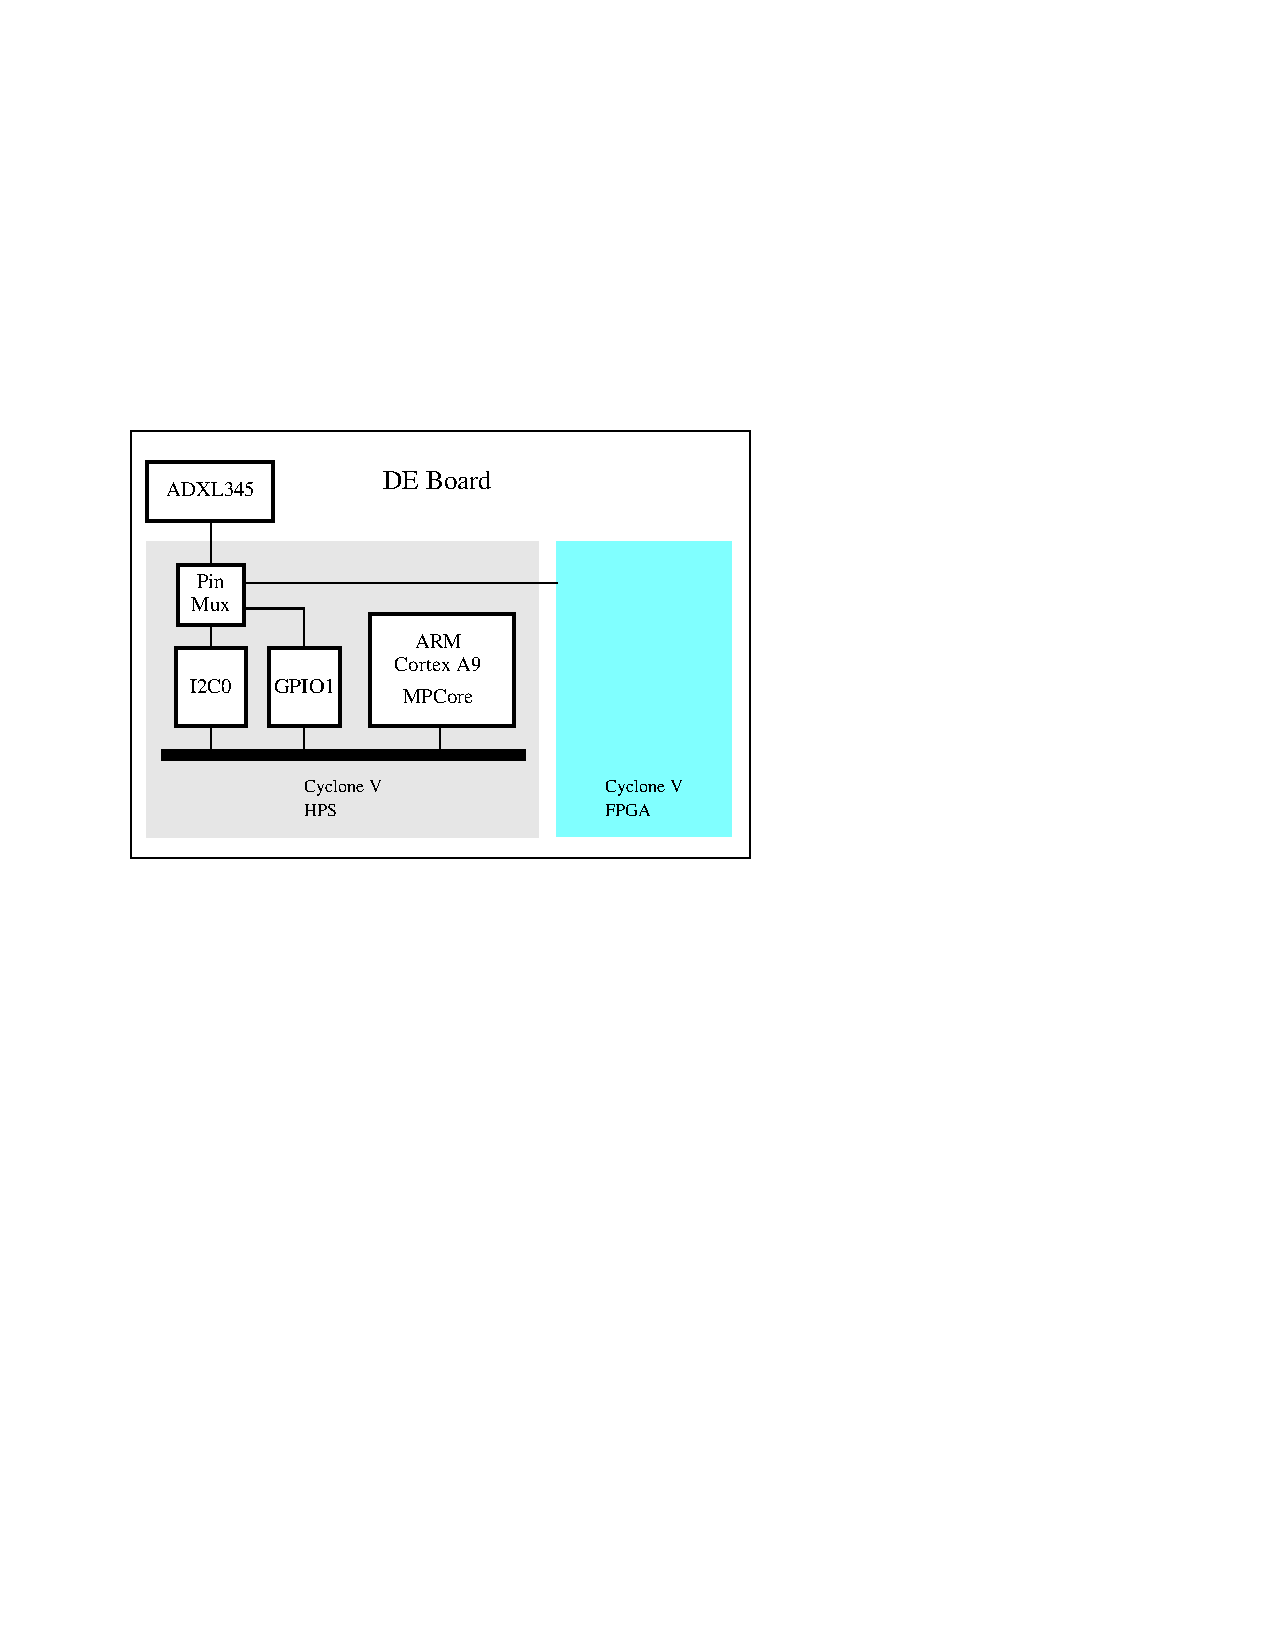
\includegraphics[scale = 1.0]{figures/fig_block_diagram_hps.pdf}
\end{center}
\caption{The ADXL345's I2C connection to the Cyclone V SoC chip on DE-Series boards.}
\label{fig:fig_block_diagram}
\end{figure}

%\subsection{Connecting the ADXL345 to the I2C0 Controller}
%\label{sec:adxl345_connection}

\begin{figure} [h]
\begin{center}
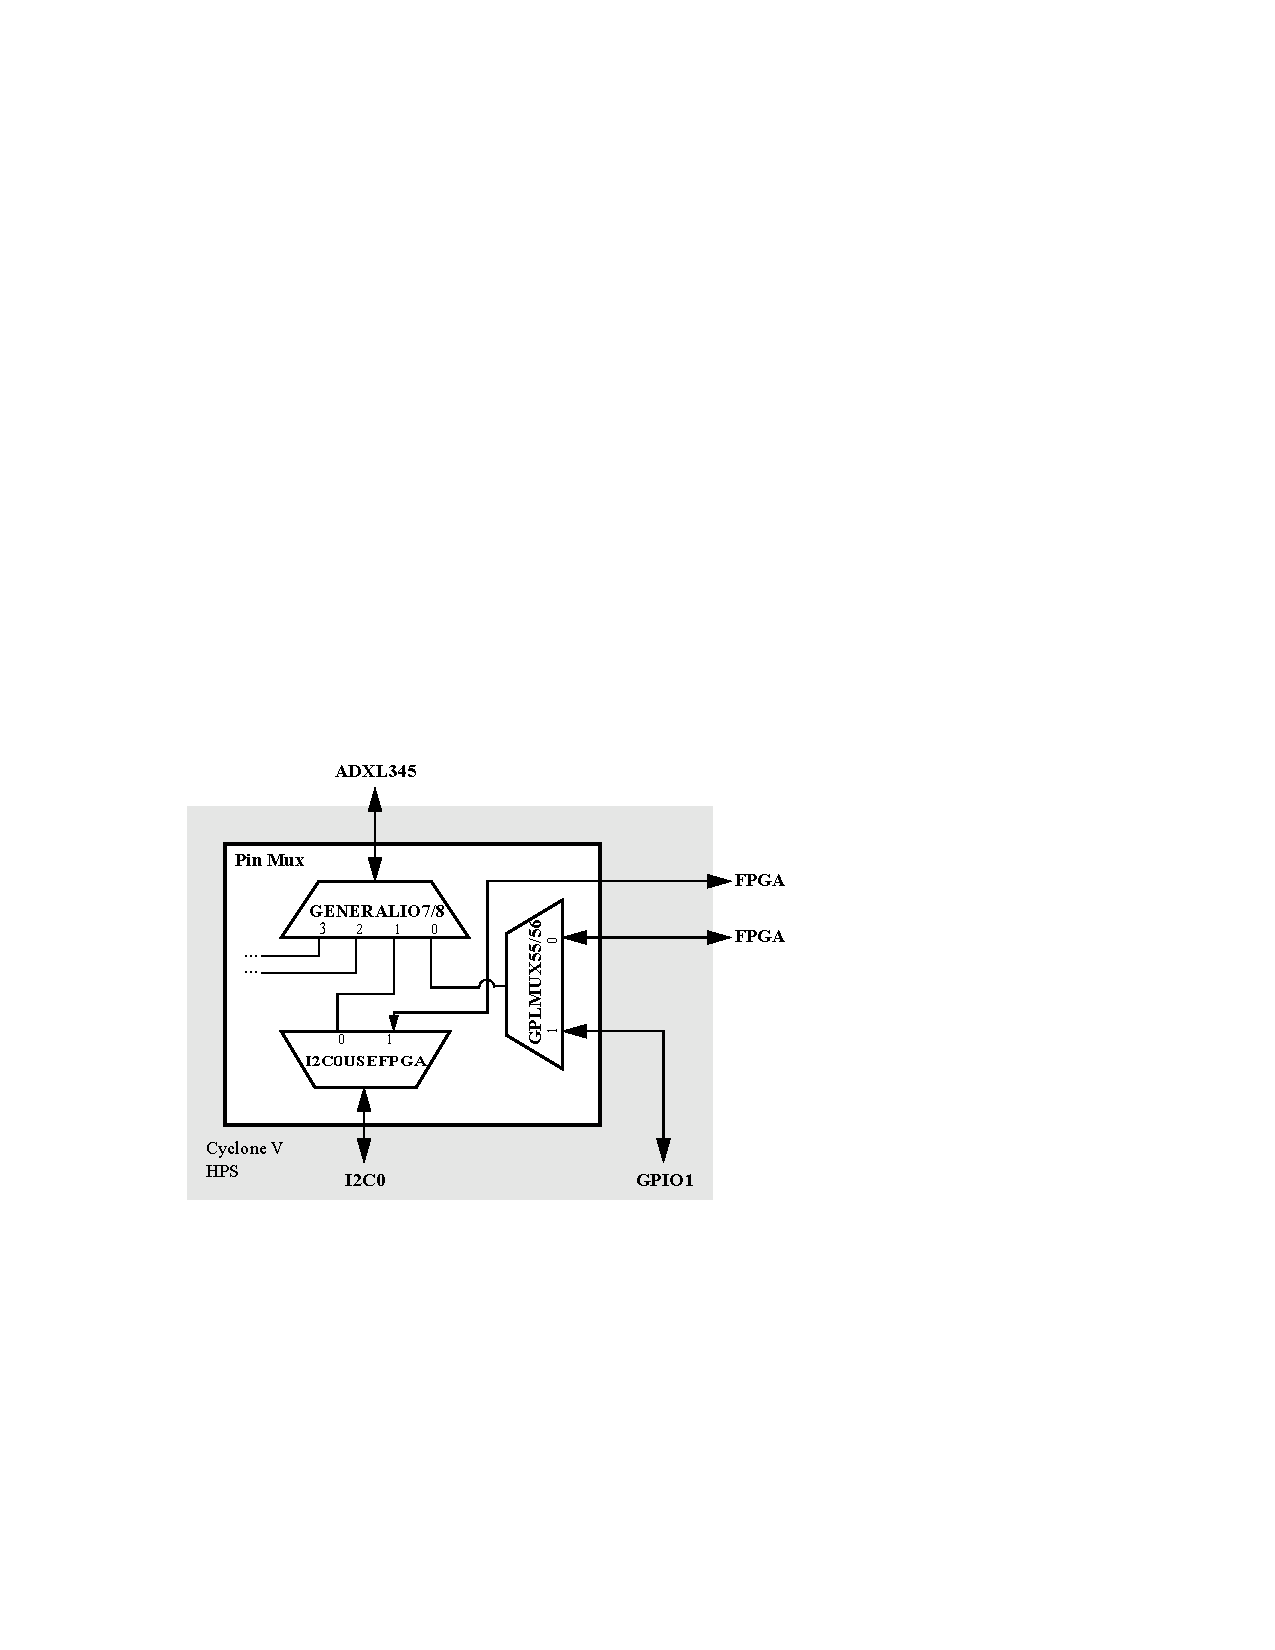
\includegraphics[scale = 1.0]{figures/fig_pinmux.pdf}
\end{center}
\caption{The Pin Mux block in more detail.}
\label{fig:pin_mux}
\end{figure}

\subsection{The Pin Multiplexer}
\label{sec:pinmux_background}

In this tutorial we will configure the Pin Mux block to route the ADXL345's I2C signals to I2C0, which is an I2C controller built into the Cyclone V HPS. As we will see in Section~\ref{sec:i2c_controller}, I2C0 provides a convenient memory-mapped register interface that makes it easy to access the ADXL345 internal registers.

\begin{table}[h]
    \centering
    \begin{tabular}{|c|c|c|c|}
        \hline
        \multicolumn{4}{|l|}{\textit{\textbf{Table 2. Pin Mux Registers*}}}
        \\\hline
            \textbf{Multiplexer}
            & \textbf{Register name}
            & \textbf{Address}
            & \textbf{Reset Value}
        \\\hline
            \multirow{2}{*}{GENERALIO7/8}
            & \texttt{GENERALIO7}
            & 0xFFD0849C
            & 0x0
        \\
            & \texttt{GENERALIO8}
            & 0xFFD084A0
            & 0x0
        \\\hline
            \multirow{2}{*}{GPLMUX55/56}
            & \texttt{GPLMUX55}
            & 0xFFD086B0
            & 0x0
        \\
            & \texttt{GPLMUX56}
            & 0xFFD086B4
            & 0x0
        \\\hline
            I2C0USEFPGA
            & \texttt{I2C0USEFPGA}
            & 0xFFD08704
            & 0x0
        \\\hline
        \multicolumn{4}{|l|}{* these registers belong to the HPS's System Manager Module}
        \\\hline
    \end{tabular}
    \label{tab:pinmux_registers}
\end{table}
%To connect the ADXL345's I2C signals to I2C0, we must configure the multiplexers inside the Pin Mux block. 
We can see from Figure~\ref{fig:pin_mux} that in order to route the I2C signals to I2C0, multiplexer GENERALIO7/8 should be configured to "1", and I2C0USEFPGA to "0". These multiplexers are controlled by memory-mapped registers, as shown in Table~\hyperref[tab:pinmux_registers]{2}.  Figure~\ref{fig:pin_muxing_code} gives C code that writes to these registers to achieve our desired routing. Note that the multiplexers GENERALIO7/8 and GPLMUX55/56 each comprise two multiplexers. While the multiplexers of each pair are controlled by registers at different addresses, they should always be configured identically. In contrast, I2C0USEFPGA is a single multiplexer, and is configured by a single register.

%Among them are the registers I2C0USEFPGA, GENERALIO7, GENERALIO8, GPLMUX55, and GPLMUX56 which control their respective multiplexers shown in Figure~\ref{fig:pin_mux}. 

%These multiplexers are controlled by the HPS's System Manager module, and to configure them we must use the System Manager's Pin Mux Control memory-mapped registers located at address 0xFFD08400. 

%Note that there are many registers in this group that control a large array of multiplexers, most of which we do not use. The registers of interest for us are

\lstset{language=C,numbers=left}
\begin{figure}[H]
\begin{center}
\begin{minipage}[t]{16 cm}
\begin{lstlisting}
#define SYSMGR_GENERALIO7   ((volatile unsigned int *) 0xFFD0849C)
#define SYSMGR_GENERALIO8   ((volatile unsigned int *) 0xFFD084A0)
#define SYSMGR_I2C0USEFPGA  ((volatile unsigned int *) 0xFFD08704)

void configure_pinmux(){
    *SYSMGR_I2C0USEFPGA = 0;
    *SYSMGR_GENERALIO7 = 1;
    *SYSMGR_GENERALIO8 = 1;
}
\end{lstlisting}
\end{minipage}
\end{center}
\vspace{-0.33in}\caption{C code that configures Pin Mux to connect the ADXL345 I2C wires to I2C0}
\label{fig:pin_muxing_code}
\end{figure}

Note that there are alternatives to using I2C0. For instance, connecting the ADXL345 to the GPIO controller (GPIO1) would allow the data pins of the GPIO to directly control the I2C wires - this could be done using software code that writes to the GPIO's data register. %Note that there are alternatives to using I2C0. For instance, connecting the ADXL345 to the GPIO controller (GPIO1) would allow your program to directly read and write the ADXL345's I2C wires using the GPIO controller's memory-mapped registers. Alternatively, you could connect the ADXL345's I2C wires to a circuit in the FPGA that is capable of communicating in the I2C protocol. %Another option would be to connect the ADXL345's I2C pins to a circuit programmed onto the FPGA which is capable of communicating in the I2C protocol. %If you wanted to manually handle I2C communication at a low level, you could route the I2C signals to the GPIO controller. The GPIO controller would then allow your program to directly read and write the SDA and SCL wires of the ADXL345's I2C interface. 

\subsection{The I2C0 Controller}
\label{sec:i2c_controller}

I2C0 is one of four I2C controllers (I2C0 - I2C3) built into the Cyclone V HPS. These generic I2C controllers are designed to be capable of communicating in the I2C serial protocol with any I2C-compatible device such as the ADXL345. These controllers provide memory-mapped register interfaces that programs can use to communicate with connected I2C devices. A benefit to using the I2C controller is that it provides a high-level interface that abstracts away many of the low-level details involved in the I2C communication protocol. %The low-level details are handled by the controller so that the user program does not have to.

We will use I2C0's memory-mapped register interface to communicate with the ADXL345. An abbreviated list of I2C0's memory-mapped registers is shown in Table~\hyperref[tab:i2c_ctrl_regtable]{3}, and further descriptions of these registers are provided in the following subsections. These registers have a width of 32 bits. 

\begin{table}[h]

    \centering
    \begin{tabular}{|c|c|c|c|p{7cm}|}
        \hline
        \multicolumn{5}{|l|}{\textit{\textbf{Table 3. I2C0 Controller Register Address Map (0xFFC04000)}}}
        \\\hline
            \textbf{Offset}
            & \textbf{Register name}
            & \textbf{Read/Write}
            & \textbf{Reset Value}
            & \textbf{Purpose}
        \\\hline
            0x0
            & \texttt{ic\_con}
            & R/W
            & 0x7D
            & Control Register
        \\\hline
            0x4
            & \texttt{ic\_tar}
            & R/W
            & 0x1055
            & Target Address Register
        \\\hline
            0x10
            & \texttt{ic\_data\_cmd}
            & R/W
            & 0x0
            & Tx Rx Data and Command Register
        \\\hline
            0x1C
            & \texttt{ic\_fs\_scl\_hcnt}
            & R/W
            & 0x3C
            & SCL High Count Register (Fast Speed)
        \\\hline
            0x20
            & \texttt{ic\_fs\_scl\_lcnt}
            & R/W
            & 0x82
            & SCL Low Count Register (Fast Speed)
        \\\hline
            0x40
            & \texttt{ic\_clr\_intr}
            & R
            & 0x0
            & Clear All Interrupts Register
        \\\hline
            0x6C
            & \texttt{ic\_enable}
            & R/W
            & 0x0
            & Enable Register
        \\\hline
            0x74
            & \texttt{ic\_txflr}
            & R
            & 0x0
            & Transmit FIFO Level Register
        \\\hline
            0x78
            & \texttt{ic\_rxflr}
            & R
            & 0x0
            & Receive FIFO Level Register
        \\\hline
            0x9C
            & \texttt{ic\_enable\_status}
            & R
            & 0x0
            & Enable Status Register
        \\\hline
    \end{tabular}
    \label{tab:i2c_ctrl_regtable}
\end{table}

If you would like a more detailed description of the I2C controller, refer to the document \textit{Cyclone V Device Handbook, Volume 3: Hard Processor System Technical Reference Manual}. For the complete list of I2C0's registers, refer to the document \textit{Cyclone V SoC HPS Address Map and Register Definitions}.

\subsubsection{ic\_con (0x0)}

\begin{table}[H]
    \centering
    \begin{tabular}{|l|l|l|l|}
        \hline
            \textbf{Bit}
            & \textbf{Name}
            & \textbf{Access}
            & \textbf{Reset}
        \\\hline
            31 - 7
            & \multicolumn{3}{|c|}{Reserved}
        \\\hline
            6
            & \texttt{ic\_slave\_disable}
            & RW
            & 0x1
        \\\hline
            5
            & \texttt{ic\_restart\_en}
            & RW
            & 0x1
        \\\hline
            4
            & \texttt{ic\_10bitaddr\_master}
            & RW
            & 0x1
        \\\hline
            3
            & \texttt{ic\_10bitaddr\_slave}
            & RW
            & 0x1
        \\\hline
            2 - 1
            & \texttt{speed}
            & RW
            & 0x2
        \\\hline
            0
            & \texttt{master\_mode}
            & RW
            & 0x1
        \\\hline
    \end{tabular}
\end{table}

This register is used to set the operating mode of I2C0. The \texttt{master\_mode} bit controls whether I2C0 acts as an I2C master or slave. A value of 0x1 selects master mode, and 0x0 selects slave mode. The \texttt{speed} bits control whether I2C0 operates in fast mode (400 kbit/s) or slow mode (100 kbit/s). The value of 0x2 selects fast mode and 0x1 selects slow mode. The \texttt{ic\_10bitaddr\_slave} and \texttt{ic\_10bitaddr\_master} bits select whether I2C0 uses 7-bit or 10-bit addressing when functioning as a slave or a master, respectively. The value of 0x0 selects 7-bit addressing, and 0x1 selects 10-bit addressing. The \texttt{ic\_restart\_en} bit enables or disables sending the restart condition to the I2C slave, when I2C0 acts as a master. The \texttt{ic\_slave\_disable} bit controls whether I2C0 should function as a slave, and should be set to 0x1 when I2C0 should act as a master, and 0x0 when it should act as a slave.

\pagebreak

For our purposes, we write 0x65 to this register. This configures I2C0 to:
\vspace{-5mm}
\begin{itemize} \itemsep0pt \parskip0pt \parsep0pt
	\item function as an I2C master
	\item run in fast mode (400 kbit/s)
	\item use 7-bit addressing mode, which is the addressing mode supported by the ADXL345
	\item use restart conditions, since this feature is supported by the ADXL345
\end{itemize}

%, we write 0x1 to \texttt{master\_mode} as we want I2C0 to act as the master to the ADXL345 slave. We write 0x2 to \texttt{speed} to select the fast mode (400 kbit/s). We write 0x0 to bit 4 since the ADXL345 supports 7-bit addressing. We also write 0x1 to \texttt{ic\_restart\_en}, as the ADXL345 supports this feature. Finally, we write 0x1 to \texttt{ic\_slave\_disable} since we want I2C0 to function as the master.

\subsubsection{ic\_tar (0x4)}

\begin{table}[H]
    \centering
    \begin{tabular}{|l|l|l|l|}
        \hline
            \textbf{Bit}
            & \textbf{Name}
            & \textbf{Access}
            & \textbf{Reset}
        \\\hline
            31 - 13
            & \multicolumn{3}{|c|}{Reserved}
        \\\hline
            12
            & \texttt{ic\_10bitaddr\_master}
            & RW
            & 0x1
        \\\hline
            11
            & \texttt{special}
            & RW
            & 0x0
        \\\hline
            10
            & \texttt{gc\_or\_start}
            & RW
            & 0x0
        \\\hline
            9 - 0
            & \texttt{ic\_tar}
            & RW
            & 0x55
        \\\hline
    \end{tabular}
\end{table}

This register is used to configure I2C0's communication with a slave. The target slave is selected by writing its slave address to the \texttt{ic\_tar} bits. The \texttt{ic\_10bitaddr\_master} bit controls whether I2C0 uses 7-bit or 10-bit addressing mode when addressing the slave. Writing 0x1 to this bit selects 10-bit addressing, while writing 0x0 selects 7-bit addressing. For our purposes, we write 0x53 (the slave address of the ADXL345) to \texttt{ic\_tar} and set \texttt{ic\_10bitaddr\_master} to 0x0, as the ADXL345 supports 7-bit addressing. The \texttt{gc\_or\_start} and \texttt{special} bits are not useful for our purposes. 

\subsubsection{ic\_data\_cmd (0x10)}

\begin{table}[H]
    \centering
    \begin{tabular}{|l|l|l|l|}
        \hline
            \textbf{Bit}
            & \textbf{Name}
            & \textbf{Access}
            & \textbf{Reset}
        \\\hline
            31 - 11
            & \multicolumn{3}{|c|}{Reserved}
        \\\hline
            10
            & \texttt{restart}
            & W
            & 0x0
        \\\hline
            9
            & \texttt{stop}
            & W
            & 0x0
        \\\hline
            8
            & \texttt{cmd}
            & W
            & 0x0
        \\\hline
            7 - 0
            & \texttt{dat}
            & RW
            & 0x0
        \\\hline
    \end{tabular}
\end{table}

This register is used to send or receive a byte to or from the ADXL345. When sending, the byte is written to \texttt{dat}, along with a 0x0 to \texttt{cmd}. When receiving, a 0x1 is first written to \texttt{cmd}, which sends a read request to the ADXL345. Once the ADXL345 replies with a byte, it can be read from \texttt{dat}. The \texttt{stop} bit is set to 0x1 when a stop signal should be sent after the byte. The \texttt{restart} bit is set to 0x1 when a restart signal should be sent before the byte. Note that \texttt{stop}, \texttt{restart}, \texttt{cmd} and \texttt{dat} are written together; a stop or restart signal cannot be sent independently of a byte.

\pagebreak

\subsubsection{ic\_fs\_scl\_hcnt (0x1C)}

\begin{table}[H]
    \centering
    \begin{tabular}{|l|l|l|l|}
        \hline
            \textbf{Bit}
            & \textbf{Name}
            & \textbf{Access}
            & \textbf{Reset}
        \\\hline
            31 - 16
            & \multicolumn{3}{|c|}{Reserved}
        \\\hline
            15 - 0
            & \texttt{ic\_fs\_scl\_hcnt}
            & RW
            & 0x3C
        \\\hline
    \end{tabular}
\end{table}

This register is used to configure the serial clock signal (SCL) that is used for synchronizing data bits sent/received by I2C0. The \texttt{ic\_fs\_scl\_hcnt} register sets the SCL clock's high period when running in the 400 kbit/s (fast) mode. The value written to this register corresponds to the number of cycles of the input clock to the I2C0 for which the SCL should remain high in each SCL clock period. The input clock to the ADXL345 is controlled the HPS, and is by default 100 MHz. We set the content of this register to 90, as described in Section~\ref{sec:configure_i2c0}.

\subsubsection{ic\_fs\_scl\_lcnt (0x20)}

\begin{table}[H]
    \centering
    \begin{tabular}{|l|l|l|l|}
        \hline
            \textbf{Bit}
            & \textbf{Name}
            & \textbf{Access}
            & \textbf{Reset}
        \\\hline
            31 - 16
            & \multicolumn{3}{|c|}{Reserved}
        \\\hline
            15 - 0
            & \texttt{ic\_fs\_scl\_lcnt}
            & RW
            & 0x82
        \\\hline
    \end{tabular}
\end{table}

This register is used to configure the serial clock signal (SCL) that is used for synchronizing data bits sent/received by I2C0. The \texttt{ic\_fs\_scl\_lcnt} register sets the SCL clock's low period when running in the 400 kbit/s (fast) mode. The value written to this register corresponds to the number of cycles of the input clock to the I2C0 for which the SCL should remain low in each SCL clock period. The input clock to the ADXL345 is controlled the HPS, and is by default 100 MHz. We set the content of this register to 160, as described in Section~\ref{sec:configure_i2c0}.%This register is used to configure the SCL clock's low period when running in the 400 kbit/s (fast) mode. The value written to this register corresponds to the the number of cycles of the input clock to the I2C0 for which the SCL should remain low in each SCL clock period. The input clock to the ADXL345 is controlled by PLLs in the HPS, and is by default 100 MHz.

\subsubsection{ic\_clr\_intr (0x40)}

\begin{table}[H]
    \centering
    \begin{tabular}{|l|l|l|l|}
        \hline
            \textbf{Bit}
            & \textbf{Name}
            & \textbf{Access}
            & \textbf{Reset}
        \\\hline
            31 - 1
            & \multicolumn{3}{|c|}{Reserved}
        \\\hline
            0
            & \texttt{clr\_intr}
            & R
            & 0x82
        \\\hline
    \end{tabular}
\end{table}

This register is used to clear software-clearable interrupts. A read of this register triggers the clear. For our purposes, we read this register when first initializing the I2C0 to clear any currently-pending interrupts.

\subsubsection{ic\_enable (0x6C)}

\begin{table}[H]
    \centering
    \begin{tabular}{|l|l|l|l|}
        \hline
            \textbf{Bit}
            & \textbf{Name}
            & \textbf{Access}
            & \textbf{Reset}
        \\\hline
            31 - 2
            & \multicolumn{3}{|c|}{Reserved}
        \\\hline
            1
            & \texttt{txabort}
            & RW
            & 0x0
        \\\hline
            0
            & \texttt{enable}
            & RW
            & 0x0
        \\\hline
    \end{tabular}
\end{table}

This register is used to enable or disable I2C communication. A 0x1, or 0x0, is written to \texttt{enable} to enable, or disable, I2C communication, respectively. A 0x1 is written to \texttt{txabort} to abort any pending transmissions.

\subsubsection{ic\_txflr (0x74)}

\begin{table}[H]
    \centering
    \begin{tabular}{|l|l|l|l|}
        \hline
            \textbf{Bit}
            & \textbf{Name}
            & \textbf{Access}
            & \textbf{Reset}
        \\\hline
            31 - 7
            & \multicolumn{3}{|c|}{Reserved}
        \\\hline
            6 - 0
            & \texttt{txflr}
            & R
            & 0x0
        \\\hline
    \end{tabular}
\end{table}

This register reports the number of valid data entries currently in I2C0's transmit FIFO buffer. When \texttt{txflr} is greater than 0, it means that there are bytes waiting to be sent to the ADXL345.

\subsubsection{ic\_rxflr (0x78)}

\begin{table}[H]
    \centering
    \begin{tabular}{|l|l|l|l|}
        \hline
            \textbf{Bit}
            & \textbf{Name}
            & \textbf{Access}
            & \textbf{Reset}
        \\\hline
            31 - 7
            & \multicolumn{3}{|c|}{Reserved}
        \\\hline
            6 - 0
            & \texttt{rxflr}
            & R
            & 0x0
        \\\hline
    \end{tabular}
\end{table}

This register reports the number of valid data entries currently in I2C0's receive FIFO buffer. When \texttt{rxflr} is greater than 0, it means that there are bytes that I2C0 has received from the ADXL345 that we have not yet read.

\subsubsection{ic\_enable\_status (0x9C)}

\begin{table}[H]
    \centering
    \begin{tabular}{|l|l|l|l|}
        \hline
            \textbf{Bit}
            & \textbf{Name}
            & \textbf{Access}
            & \textbf{Reset}
        \\\hline
            31 - 3
            & \multicolumn{3}{|c|}{Reserved}
        \\\hline
            2
            & \texttt{slv\_rx\_data\_lost}
            & R
            & 0x0
        \\\hline
            1
            & \texttt{slv\_disabled\_while\_busy}
            & R
            & 0x0
        \\\hline
            0
            & \texttt{ic\_en}
            & R
            & 0x0
        \\\hline
    \end{tabular}
\end{table}

This register is used to check whether I2C0 has reached the enabled state. After writing a 0x1 to the \texttt{enable} bit in the \texttt{ic\_enable} register, we poll this register until the \texttt{ic\_en} bit becomes 0x1, signalling that I2C0 is ready for operation. Similarly, after writing a 0x0 to the \texttt{enable} bit, we poll until \texttt{ic\_en} becomes 0x0, signalling that I2C0 has been disabled.

\pagebreak
\section{Using the Accelerometer in C-Language Code}
\label{sec:using_accel_in_code}

The following sections provide C-language code for configuring and operating the ADXL345, the I2C0 controller, and the Pin Multiplexer block. This code can also be found in the files \texttt{ADXL345.c} and \texttt{ADXL345.h} which accompany this tutorial. The code should be compiled, loaded, and executed using the \productNameMed{}. If you are not familiar with the \productNameMed{} you can refer to the document \textit{\productNameMed{} Tutorial}. %The code can be found in the files \texttt{ADXL345.c} and \texttt{ADXL345.h} which accompany this tutorial.

\subsection{Configuring the Pin Multiplexer}

As described in Section~\ref{sec:pinmux_background}, the first step in using the ADXL345 is to configure the Pin Mux block in the Cyclone V HPS to connect the ADXL345's I2C wires to I2C0. Figure~\ref{fig:pin_muxing_code_2} shows the function \texttt{Pinmux\_Config()} that accomplishes this. The function writes to the memory-mapped registers GENERALIO7, GENERALIO8, and I2C0USEFPGA which control multiplexers inside the Pin Mux block (shown in Figure~\ref{fig:pin_mux}).

\lstset{language=C,numbers=left}
\begin{figure}[H]
\begin{center}
\begin{minipage}[t]{16 cm}
\begin{lstlisting}
void Pinmux_Config(){
    *SYSMGR_I2C0USEFPGA = 0;
    *SYSMGR_GENERALIO7 = 1;
    *SYSMGR_GENERALIO8 = 1;
}
\end{lstlisting}
\end{minipage}
\end{center}
\vspace{-0.33in}\caption{C code that configures Pin Mux to connect the ADXL345's I2C wires to I2C0}
\label{fig:pin_muxing_code_2}
\end{figure}

\subsection{Configuring I2C0}
\label{sec:configure_i2c0}

Once the ADXL345's I2C wires are connected to I2C0, you must configure I2C0 for communication with the ADXL345. Figure~\ref{fig:i2c0_init_code} shows the function \texttt{I2C0\_Init()} that configures I2C0 with the appropriate settings. Important lines of the code are described below:
%\vspace{-5mm}
%\begin{itemize} \itemsep0pt \parskip0pt \parsep0pt
\begin{itemize} \itemsep0.5pt
\item Line 4 aborts any pending transmissions and disables I2C0. This is required before modifying any of I2C0's settings.
\item Line 7 polls the enable status register until the I2C0 is fully disabled. 
\item Line 11 writes 0x65 to I2C0\_CON, which configures I2C0 to:
	\begin{itemize} \itemsep0.5pt
	\item function as an I2C master. It will control the ADXL345, which functions as the slave.
	\item run in fast mode (400 kbit/s), as supported by the ADXL345.
	\item use 7-bit addressing mode, as required by the ADXL345.
	\item use restart conditions, as supported by the ADXL345. 
	\end{itemize}
\item Line 14 writes 0x53 to I2C0\_TAR, which configures I2C0 to target the ADXL345.
\item Lines 19 and 20 configure the SCL clock that will drive the ADXL345. The ADXL345 requires the SCL clock period to be at least 2.5 $\mu$s, the SCL high time to be at least 0.6 $\mu$s, and the SCL low time to be at least 1.3 $\mu$s. All three conditions are met by setting the high period to be 0.9 $\mu$s (90 cycles of the 100 MHz input clock to I2C0), and setting the low period to be 1.6 $\mu$s (160 cycles of the 100 MHz input clock to I2C0).
\item Line 23 re-enables I2C0 now that all settings have been configured, and Line 26 waits until I2C0 reaches its operational state.
\end{itemize}

%First, it disables I2C0 by writing 0 to I2C0\_ENABLE. This is required before modifying any of I2C0's settings. Then it write 0x65 to I2C0\_CON, which configures I2C0 to:
%\vspace{-5mm}
%\begin{itemize} \itemsep0pt \parskip0pt \parsep0pt
%	\item function as an I2C master. It will control ADXL345, which functions as the slave.
%	\item run in fast mode (400 kbit/s), as supported by the ADXL345.
%	\item use 7-bit addressing mode. This is the addressing mode supported by the ADXL345.
%	\item use restart conditions, as supported by the ADXL345.
%\end{itemize}
%Then it configures I2C0 to target the ADXL345 by writing 0x53 (the slave address of ADXL345) to the I2C0\_TAR register. Then the SCL clock that is sent to the ADXL345 is configured by writing to the I2C0\_FS\_SCL\_HCNT and I2C0\_FS\_SCL\_LCNT registers. 

\begin{figure}[H]
\begin{center}
\begin{minipage}[t]{16 cm}
\begin{lstlisting}
void I2C0_Init(){

    // Abort any ongoing transmits and disable I2C0.
    *I2C0_ENABLE = 2;
    
    // Wait until I2C0 is disabled
    while(((*I2C0_ENABLE_STATUS)&0x1) == 1){}
    
    // Configure the config reg with the desired setting (act as 
    // a master, use 7bit addressing, fast mode (400kb/s)).
    *I2C0_CON = 0x65;
    
    // Set target address (disable special commands, use 7bit addressing)
    *I2C0_TAR = 0x53;
    
    // Set SCL high/low counts (Assuming default 100MHZ clock input to I2C0 Controller).
    // The minimum SCL high period is 0.6us, and the minimum SCL low period is 1.3us,
    // However, the combined period must be 2.5us or greater, so add 0.3us to each.
    *I2C0_FS_SCL_HCNT = 60 + 30; // 0.6us + 0.3us
    *I2C0_FS_SCL_LCNT = 130 + 30; // 1.3us + 0.3us
    
    // Enable the controller
    *I2C0_ENABLE = 1;
    
    // Wait until controller is powered on
    while(((*I2C0_ENABLE_STATUS)&0x1) == 0){}
}
\end{lstlisting}
\end{minipage}
\end{center}
\vspace{-0.33in}\caption{A function that configures I2C0.}
\label{fig:i2c0_init_code}
\end{figure}

\pagebreak
\subsection{Reading and Writing the ADXL345 Internal Registers}

Once the ADXL345's I2C wires are routed to I2C0 and I2C0 has been configured, you can use I2C0's memory-mapped registers to read and write the ADXL345 internal registers. %\texttt{ADXL345.h} in the design files provides prewritten C functions that read and write ADXL345's internal registers through I2C0. These functions are shown below in Figures~\ref{fig:read_function},~\ref{fig:write_function}, and~\ref{fig:multi_read_function}.

The \texttt{ADXL345\_REG\_READ(uint8\_t address, uint8\_t *value)} function shown in Figure~\ref{fig:read_function} performs a read of a single internal register at internal address \texttt{address} and writes the value read into \texttt{value}. It does this in three steps. First, it sends the address of the target register, along with a START signal (line 5). Second, it sends the read request (line 8). Finally in lines 11 and 12, the function waits until I2C0 has received a response from ADXL345, then writes the value to \texttt{value}.

\begin{figure}[H]
\begin{center}
\begin{minipage}[t]{16 cm}
\begin{lstlisting}
// Read value from internal register at address
void ADXL345_REG_READ(uint8_t address, uint8_t *value){

    // Send reg address (+0x400 to send START signal)
    *I2C0_DATA_CMD = address + 0x400;
    
    // Send read signal
    *I2C0_DATA_CMD = 0x100;
    
    // Read the response (first wait until RX buffer contains data)  
    while (*I2C0_RXFLR == 0){}
    *value = *I2C0_DATA_CMD;
}
\end{lstlisting}
\end{minipage}
\end{center}
\vspace{-0.33in}\caption{A function that reads the ADXL345 internal registers.}
\label{fig:read_function}
\end{figure}

The \texttt{ADXL345\_REG\_WRITE(uint8\_t address, uint8\_t value)} function shown in Figure~\ref{fig:write_function} writes the value \texttt{value} to the internal register at address \texttt{address}. It does this in two steps. First, it sends the address of the target register, along with a START signal. Then it sends the value \texttt{value}.

\begin{figure}[H]
\begin{center}
\begin{minipage}[t]{16 cm}
\begin{lstlisting}
// Write value to internal register at address
void ADXL345_REG_WRITE(uint8_t address, uint8_t value){
    
    // Send reg address (+0x400 to send START signal)
    *I2C0_DATA_CMD = address + 0x400;
    
    // Send value
    *I2C0_DATA_CMD = value;
}
\end{lstlisting}
\end{minipage}
\end{center}
\vspace{-0.33in}\caption{A function that writes to ADXL345 internal registers.}
\label{fig:write_function}
\end{figure}

\pagebreak
The \texttt{ADXL345\_REG\_MULTI\_READ(uint8\_t address, uint8\_t values[], uint8\_t len)} function shown in Figure~\ref{fig:multi_read_function} performs a read of \texttt{len} consecutive internal registers, starting at internal address \texttt{address}. It stores the values read in the array \texttt{values}. This function is used when reading the six DATA registers inside the ADXL345, which are at consecutive addresses 0x32 - 0x37. Because this function performs a single read of multiple consecutive registers, it ensures that none of the DATA registers are modified while the read is being performed. This operation is preferable to performing multiple single reads, where the DATA registers could be modified if the ADXL345 samples its acceleration values in between the reads.

\begin{figure}[H]
\begin{center}
\begin{minipage}[t]{16 cm}
\begin{lstlisting}
// Read multiple consecutive internal registers
void ADXL345_REG_MULTI_READ(uint8_t address, uint8_t values[], uint8_t len){

    // Send reg address (+0x400 to send START signal)
    *I2C0_DATA_CMD = address + 0x400;
    
    // Send read signal len times
    int i;
    for (i=0;i<len;i++)
        *I2C0_DATA_CMD = 0x100;

    // Read the bytes
    int nth_byte=0;
    while (len){
        if ((*I2C0_RXFLR) > 0){
            values[nth_byte] = *I2C0_DATA_CMD;
            nth_byte++;
            len--;
        }
    }
}
\end{lstlisting}
\end{minipage}
\end{center}
\vspace{-0.33in}\caption{A function that reads \texttt{len} consecutive registers.}
\label{fig:multi_read_function}
\end{figure}

\subsection{Configuring the ADXL345}

The ADXL345 has various settings that can be configured to alter its operation. These settings are configured by writing to the ADXL345 control registers, which you can do using the \texttt{ADXL345\_REG\_WRITE} function.  Figure~\ref{fig:config_adxl345} shows the function \texttt{ADXL345\_Init()} which configures the ADXL345 to run in +/- 16 g mode, and sample acceleration at a rate of 100 Hz. It also configures the ADXL345 to run in full resolution mode, which forces a resolution of 3.9 mg (the least significant bit of the DATA values represents 3.9 mg).

\begin{figure}[H]
\begin{center}
\begin{minipage}[t]{16 cm}
\begin{lstlisting}
// Initialize the ADXL345 chip
void ADXL345_Init(){
    
    // +- 16g range, full resolution
    ADXL345_REG_WRITE(ADXL345_REG_DATA_FORMAT, XL345_RANGE_16G | XL345_FULL_RESOLUTION);
    
    // Output Data Rate: 200Hz
    ADXL345_REG_WRITE(ADXL345_REG_BW_RATE, XL345_RATE_200);

    // The DATA_READY bit is not reliable. It is updated at a much higher rate than the Data Rate
    // Use the Activity and Inactivity interrupts as indicators for new data.
    ADXL345_REG_WRITE(ADXL345_REG_THRESH_ACT, 0x04); //activity threshold
    ADXL345_REG_WRITE(ADXL345_REG_THRESH_INACT, 0x02); //inactivity threshold
    ADXL345_REG_WRITE(ADXL345_REG_TIME_INACT, 0x02); //time for inactivity
    ADXL345_REG_WRITE(ADXL345_REG_ACT_INACT_CTL, 0xFF); //Enables AC coupling for thresholds
    ADXL345_REG_WRITE(ADXL345_REG_INT_ENABLE, XL345_ACTIVITY | XL345_INACTIVITY );	//enable interrupts
    
    // stop measure
    ADXL345_REG_WRITE(ADXL345_REG_POWER_CTL, XL345_STANDBY);
    
    // start measure
    ADXL345_REG_WRITE(ADXL345_REG_POWER_CTL, XL345_MEASURE);
}
\end{lstlisting}
\end{minipage}
\end{center}
\vspace{-0.33in}\caption{A function that configures the ADXL345 mode of operation.}
\label{fig:config_adxl345}
\end{figure}
\vspace{-10pt}

\subsection{Reading the Acceleration Data}

Now that the ADXL345 is configured for operation, you can read acceleration data from its DATA registers. Figure~\ref{fig:read_accel_data} shows the function \texttt{ADXL345\_XYZ\_READ(int16\_t szData16[3])} which reads the acceleration for the X, Y and Z axes and stores the data in \texttt{szData16[0]}, \texttt{szData16[1]}, and \texttt{szData16[2]}, respectively. Line 5 calls \texttt{ADXL345\_REG\_MULTI\_READ} to read the ADXL345's six DATA registers. This reads two registers for each axis, one representing the bottom 8 bits and the other representing the top 8 bits of the acceleration sample. Lines 7 to 9 combine these two halves for each axis and write the 16-bit values into \texttt{szData16}. The least-significant bit of these values represents 3.9 mg, and the values range from -4096 to 4095 (a resolution of 13 bits). %In the end, the acceleration value for the X, Y, and Z axes are stored in \texttt{szData16[0]}, \texttt{szData16[1]}, and \texttt{szData16[2]}, respectively. The values are signed integers, and the least significant bit represents 3.9 mg.

\begin{figure}[H]
\begin{center}
\begin{minipage}[t]{16 cm}
\begin{lstlisting}
// Read acceleration data of all three axes
void ADXL345_XYZ_Read(int16_t szData16[3]){

    uint8_t szData8[6];
    ADXL345_REG_MULTI_READ(0x32, (uint8_t *)&szData8, sizeof(szData8));
    
    szData16[0] = (szData8[1] << 8) | szData8[0]; 
    szData16[1] = (szData8[3] << 8) | szData8[2];
    szData16[2] = (szData8[5] << 8) | szData8[4];
}
\end{lstlisting}
\end{minipage}
\end{center}
\vspace{-0.33in}\caption{A function that reads the acceleration data for the x, y, and z axes.}
\label{fig:read_accel_data}
\end{figure}

The ADXL345 is set to sample acceleration 100 times a second, which is very slow relative to a modern processor. This makes it possible for a program to read the ADXL345 far more often than 100 times each second, leading to duplicate reads of the same samples. To prevent this, we can check the \texttt{Data\_ready} bit of the ADXL345's \texttt{INT\_SOURCE} register and only call \texttt{ADXL345\_XYZ\_Read} when there is new data available. Figure~\ref{fig:check_data_ready} shows the function \texttt{ADXL345\_IsDataReady()} which checks the \texttt{Data\_ready} bit and returns true if there is new data, and false otherwise.

%Because the ADXL345 is set to sample acceleration 100 times a second, a new sample is available every 10 ms. To ensure that our program does make duplicate reads of the same acceleration sample, we can read the ADXL345's \texttt{INT\_SOURCE} register and check whether there is a new sample before calling \texttt{ADXL345\_XYZ\_Read}. The \texttt{INT\_SOURCE} register's \texttt{Data\_ready} is set to 1 whenever there is a new sample, and is cleared when the sample is read. Figure~\ref{fig:check_data_ready} shows the function \texttt{ADXL345\_IsDataReady()} which checks the \texttt{Data\_ready} bit and returns true if there is new data, and false otherwise.

\begin{figure}[H]
\begin{center}
\begin{minipage}[t]{16 cm}
\begin{lstlisting}
// Return true if there is new data
bool ADXL345_IsDataReady(){
    bool bReady = false;
    uint8_t data8;
    
    ADXL345_REG_READ(ADXL345_REG_INT_SOURCE,&data8);
    if (data8 & XL345_ACTIVITY)
        bReady = true;
    
    return bReady;
}
\end{lstlisting}
\end{minipage}
\end{center}
\vspace{-0.33in}\caption{A function that checks if there is new acceleration data.}
\label{fig:check_data_ready}
\end{figure}

\subsection{Putting it All Together: An Example C Program}

\lstset{language=C,numbers=left}
\begin{figure}[h]
\begin{center}
\begin{minipage}[t]{16 cm}
\begin{lstlisting}
#include "ADXL345.h"
#include <stdio.h>

int main(void){

    uint8_t devid;
    int16_t mg_per_lsb = 4;
    int16_t XYZ[3];
    
    // Configure Pin Muxing
    Pinmux_Config();
    
    // Initialize I2C0 Controller
    I2C0_Init();
    
    // 0xE5 is read from DEVID(0x00) if I2C is functioning correctly
    ADXL345_REG_READ(0x00, &devid);
    
    // Correct Device ID
    if (devid == 0xE5){
        // Initialize accelerometer chip
        ADXL345_Init();
        
        while(1){
            if (ADXL345_IsDataReady()){
                ADXL345_XYZ_Read(XYZ);
                printf("X=%d mg, Y=%d mg, Z=%d mg\n", XYZ[0]*mg_per_lsb, XYZ[1]*mg_per_lsb, XYZ[2]*mg_per_lsb);
            }
        }
    } else {
        printf("Incorrect device ID\n");
    }
    
    return 0;
}
\end{lstlisting}
\end{minipage}
\end{center}
\vspace{-0.33in}\caption{C code that reads acceleration data from the ADXL345}
\label{fig:arm_c_code}
\end{figure}

Figure~\ref{fig:arm_c_code} shows a simple program that calls the functions described in the previous sections to initialize the required components and then loops forever to read and print out acceleration data. Important lines of the code are explained below:

\begin{itemize} \itemsep0.5pt
\item Line 1 includes the header file \texttt{ADXL345.h}, which contains all of the functions for working with the ADXL345 and the I2C0 controller. 
\item Line 11 calls the function \texttt{Pinmux\_Config()} which configures the Pin Mux block to connect the ADXL345's I2C wires to I2C0.
\item Line 14 calls the function \texttt{I2C0\_Init()} which configures the I2C0 controller to communicate with the ADXL345 chip. 
\item Line 17 reads the Device ID internal register of the ADXL345 chip. If the I2C communication is working correctly, the device ID 0xE5 is read.
\item Line 22 calls the function \texttt{ADXL345\_Init()} which configures the ADXL345 chip to start measuring acceleration data.
\item Line 26 calls the function \texttt{ADXL345\_XYZ\_Read(XYZ)} which reads the acceleration data for all three axes, and stores the data in the XYZ array. The least significant bit of the acceleration values read from the ADXL345 represent 3.9 mg increments (approximately 0.038 m/s$^2$, since g = 9.81 m/s$^2$). To account for this when printing out the data in line 23, the values are multiplied by \texttt{mg\_per\_lsb} to output numbers in mg units. 
\end{itemize}
%Line 1 includes the \texttt{ADXL345.h} header file, which provides various functions for working with the ADXL345 and the I2C0 controller. Line 11 calls the function \texttt{I2C0\_Init()} which configures the I2C0 controller to communicate with the ADXL345 chip. Line 14 calls the function \texttt{ADXL345\_Init()} which configures the ADXL345 chip to start measuring acceleration data. Line 17 calls the function \texttt{ADXL345\_IdRead(pid)}, which reads the Device ID internal register of the ADXL345 chip, and writes the value into \texttt{pid}. If the I2C communication is working correctly, the device ID 0xE5 should be read. 

%Line 22 calls the function \texttt{ADXL345\_XYZ\_Read(XYZ)} which reads the acceleration data for all three axes, and stores the data in the XYZ array. The least significant bit of the acceleration values read from the ADXL345 represent 3.9 mg increments (approximately 0.038 m/s$^2$, since g = 9.81 m/s$^2$). Thus, when printing out the data in line 23, the values are multiplied by \texttt{mg\_per\_lsb} to output numbers as mg. 


% Copyright and Trademark

%\newcommand{\datePublished}{Mar 2022}

\newcommand{\versnum}{21.1} %version number quartus/AMP
\newcommand{\quartusname}{Quartus\textsuperscript{\textregistered} Prime}	
\newcommand{\textBar}{For \quartusname{} \versnum{}}
\newcommand{\thisyear}{2022 } %for copyright
\newcommand{\company}{FPGAcademy.org}
\newcommand{\longteamname}{FPGAcademy.org}
\newcommand{\teamname}{FPGAcademy}
\newcommand{\website}{FPGAcademy.org}

\newcommand{\productAcronym}{AMP}
\newcommand{\productNameShort}{Monitor Program}

\newcommand{\productNameMedTM}{Monitor Program}
\newcommand{\productNameMed}{Monitor Program}

%\newcommand{\headerLogoFilePath}[1]{#1/FPGAcademy.png}



%%%%%%%%%%%%%%%%%%%%%%%%%%%%%%%%%%%%%%%%
%%% FPGAcademy Copyright Information %%%
%%%%%%%%%%%%%%%%%%%%%%%%%%%%%%%%%%%%%%%%

%Always put the copyright on a new page (clear page), with some vertical space from top
\clearpage
\vspace{1in}

\noindent

Copyright {\copyright} FPGAcademy.org. All rights reserved. FPGAcademy and the FPGAcademy logo are trademarks of  FPGAcademy.org.  This document is being provided on an ``as-is'' basis and as an accommodation and therefore all warranties, representations or guarantees of any kind (whether express, implied or statutory) including, without limitation, warranties of merchantability, non-infringement, or fitness for a particular purpose, are specifically disclaimed.

%FPGAcademy assumes no responsibility or liability arising out of the application or use of any information,  product,  or  service  described  herein  except  as  expressly  agreed  to  in  writing  by  FPGAcademy.



**Other names and brands may be claimed as the property of others.



\end{document}

